\begin{figure}[tp]
	\centering
	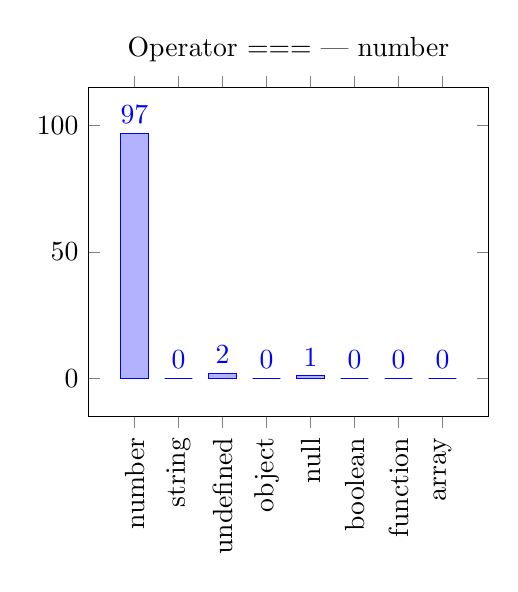
\begin{tikzpicture}
		\begin{axis}[
			ybar,
			title=Operator ${===}$ | number,
			width=0.55\textwidth,
			ybar=0pt,
			ymax=100,
			enlargelimits=0.15,
			legend style={at={(0.5,-0.2)}, anchor=north,legend columns=-1},
			symbolic x coords={number,string,undefined,object,null,boolean,function,array},
			xtick=data,
			nodes near coords, 
			nodes near coords align={vertical},
			x tick label style={rotate=90,anchor=east},
		]
		\addplot coordinates {
			(number, 97)
			(string, 0)
			(undefined, 2)
			(object, 0)
			(null, 1)
			(boolean, 0)
			(function, 0)
			(array, 0)
		};
		\end{axis}
	\end{tikzpicture}
	%
	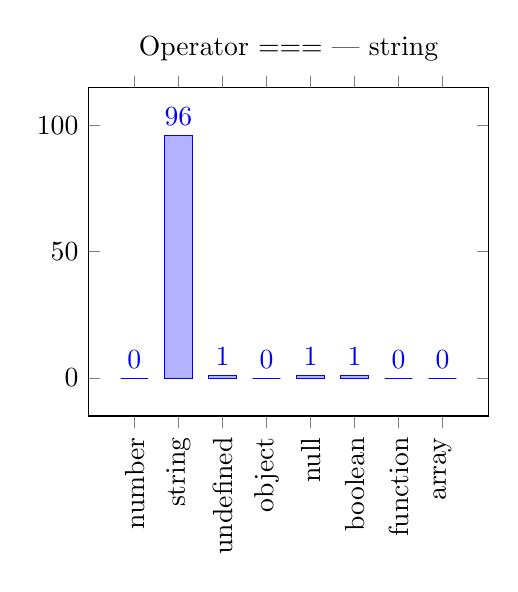
\begin{tikzpicture}
		\begin{axis}[
			ybar,
			title=Operator ${===}$ | string,
			width=0.55\textwidth,
			ybar=0pt,
			ymax=100,
			enlargelimits=0.15,
			legend style={at={(0.5,-0.2)}, anchor=north,legend columns=-1},
			symbolic x coords={number,string,undefined,object,null,boolean,function,array},
			xtick=data,
			nodes near coords, 
			nodes near coords align={vertical},
			x tick label style={rotate=90,anchor=east},
		]
		\addplot coordinates {
			(number, 0)
			(string, 96)
			(undefined, 1)
			(object, 0)
			(null, 1)
			(boolean, 1)
			(function, 0)
			(array, 0)
		};
		\end{axis}
	\end{tikzpicture}
	%
	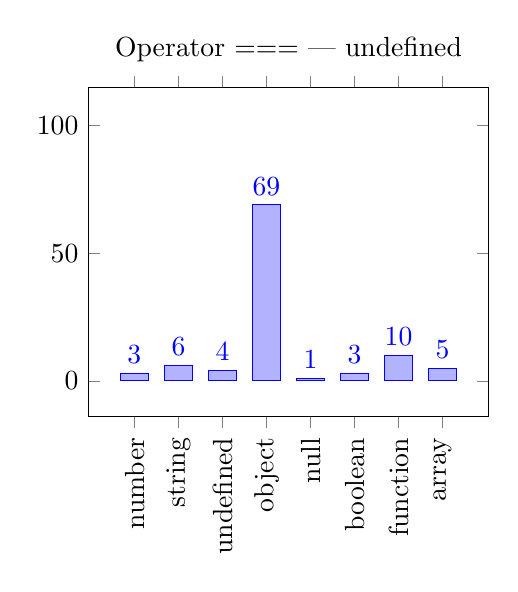
\begin{tikzpicture}
		\begin{axis}[
			ybar,
			title=Operator ${===}$ | undefined,
			width=0.55\textwidth,
			ybar=0pt,
			ymax=100,
			enlargelimits=0.15,
			legend style={at={(0.5,-0.2)}, anchor=north,legend columns=-1},
			symbolic x coords={number,string,undefined,object,null,boolean,function,array},
			xtick=data,
			nodes near coords, 
			nodes near coords align={vertical},
			x tick label style={rotate=90,anchor=east},
		]
		\addplot coordinates {
			(number, 3)
			(string, 6)
			(undefined, 4)
			(object, 69)
			(null, 1)
			(boolean, 3)
			(function, 10)
			(array, 5)
		};
		\end{axis}
	\end{tikzpicture}
	%
	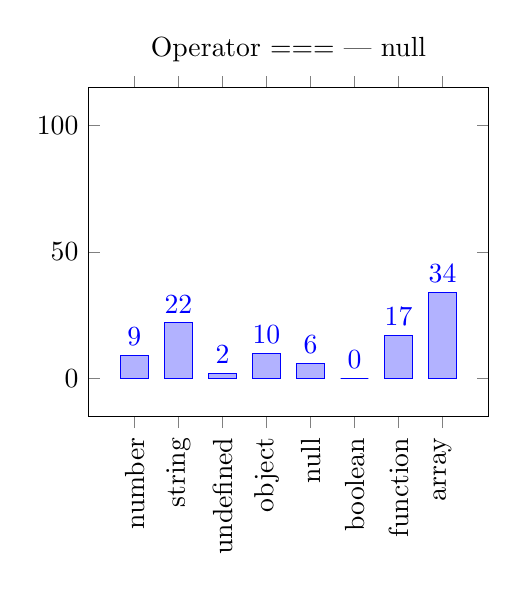
\begin{tikzpicture}
		\begin{axis}[
			ybar,
			title=Operator ${===}$ | null,
			width=0.55\textwidth,
			ybar=0pt,
			ymax=100,
			enlargelimits=0.15,
			legend style={at={(0.5,-0.2)}, anchor=north,legend columns=-1},
			symbolic x coords={number,string,undefined,object,null,boolean,function,array},
			xtick=data,
			nodes near coords, 
			nodes near coords align={vertical},
			x tick label style={rotate=90,anchor=east},
		]
		\addplot coordinates {
			(number, 9)
			(string, 22)
			(undefined, 2)
			(object, 10)
			(null, 6)
			(boolean, 0)
			(function, 17)
			(array, 34)
		};
		\end{axis}
	\end{tikzpicture}

	\caption[Usage distribution for operator ===]{\textbf{Usage distribution for operator \mintinline{text}{===}} - All graphs were made by fixing the type of one of the operands. That means, for example, that if a value is used with the operator \mintinline{text}{===} and the other operand is a \mintinline{text}{number}, the top-left graph should be used.}
	\label{fig:type-inference-proposal-scoring-strict-equal}
\end{figure}